\documentclass[12pt]{report}

\usepackage[T1]{fontenc} 
\usepackage[utf8]{inputenc}
\usepackage[francais]{babel}
\usepackage{graphicx}


\title{Rapport - Projet technologique - Hashiwokakero}
\author{Groupe TM2H}

\begin{document}

\maketitle

\begin{abstract}
Ceci est le résumé du rapport.
\end{abstract}

\tableofcontents

\section{Implantation de la librarie hashi}

\subsection{Création des fonctions de base}

\subsubsection{Les fonctions de game.c}

\subsubsection{Les fonctions de node.c}

\subsection{Création d'un affichage terminal}
\section{Extension de la librarie hashi sur 8 directions}
\newpage
\section{Solveur}

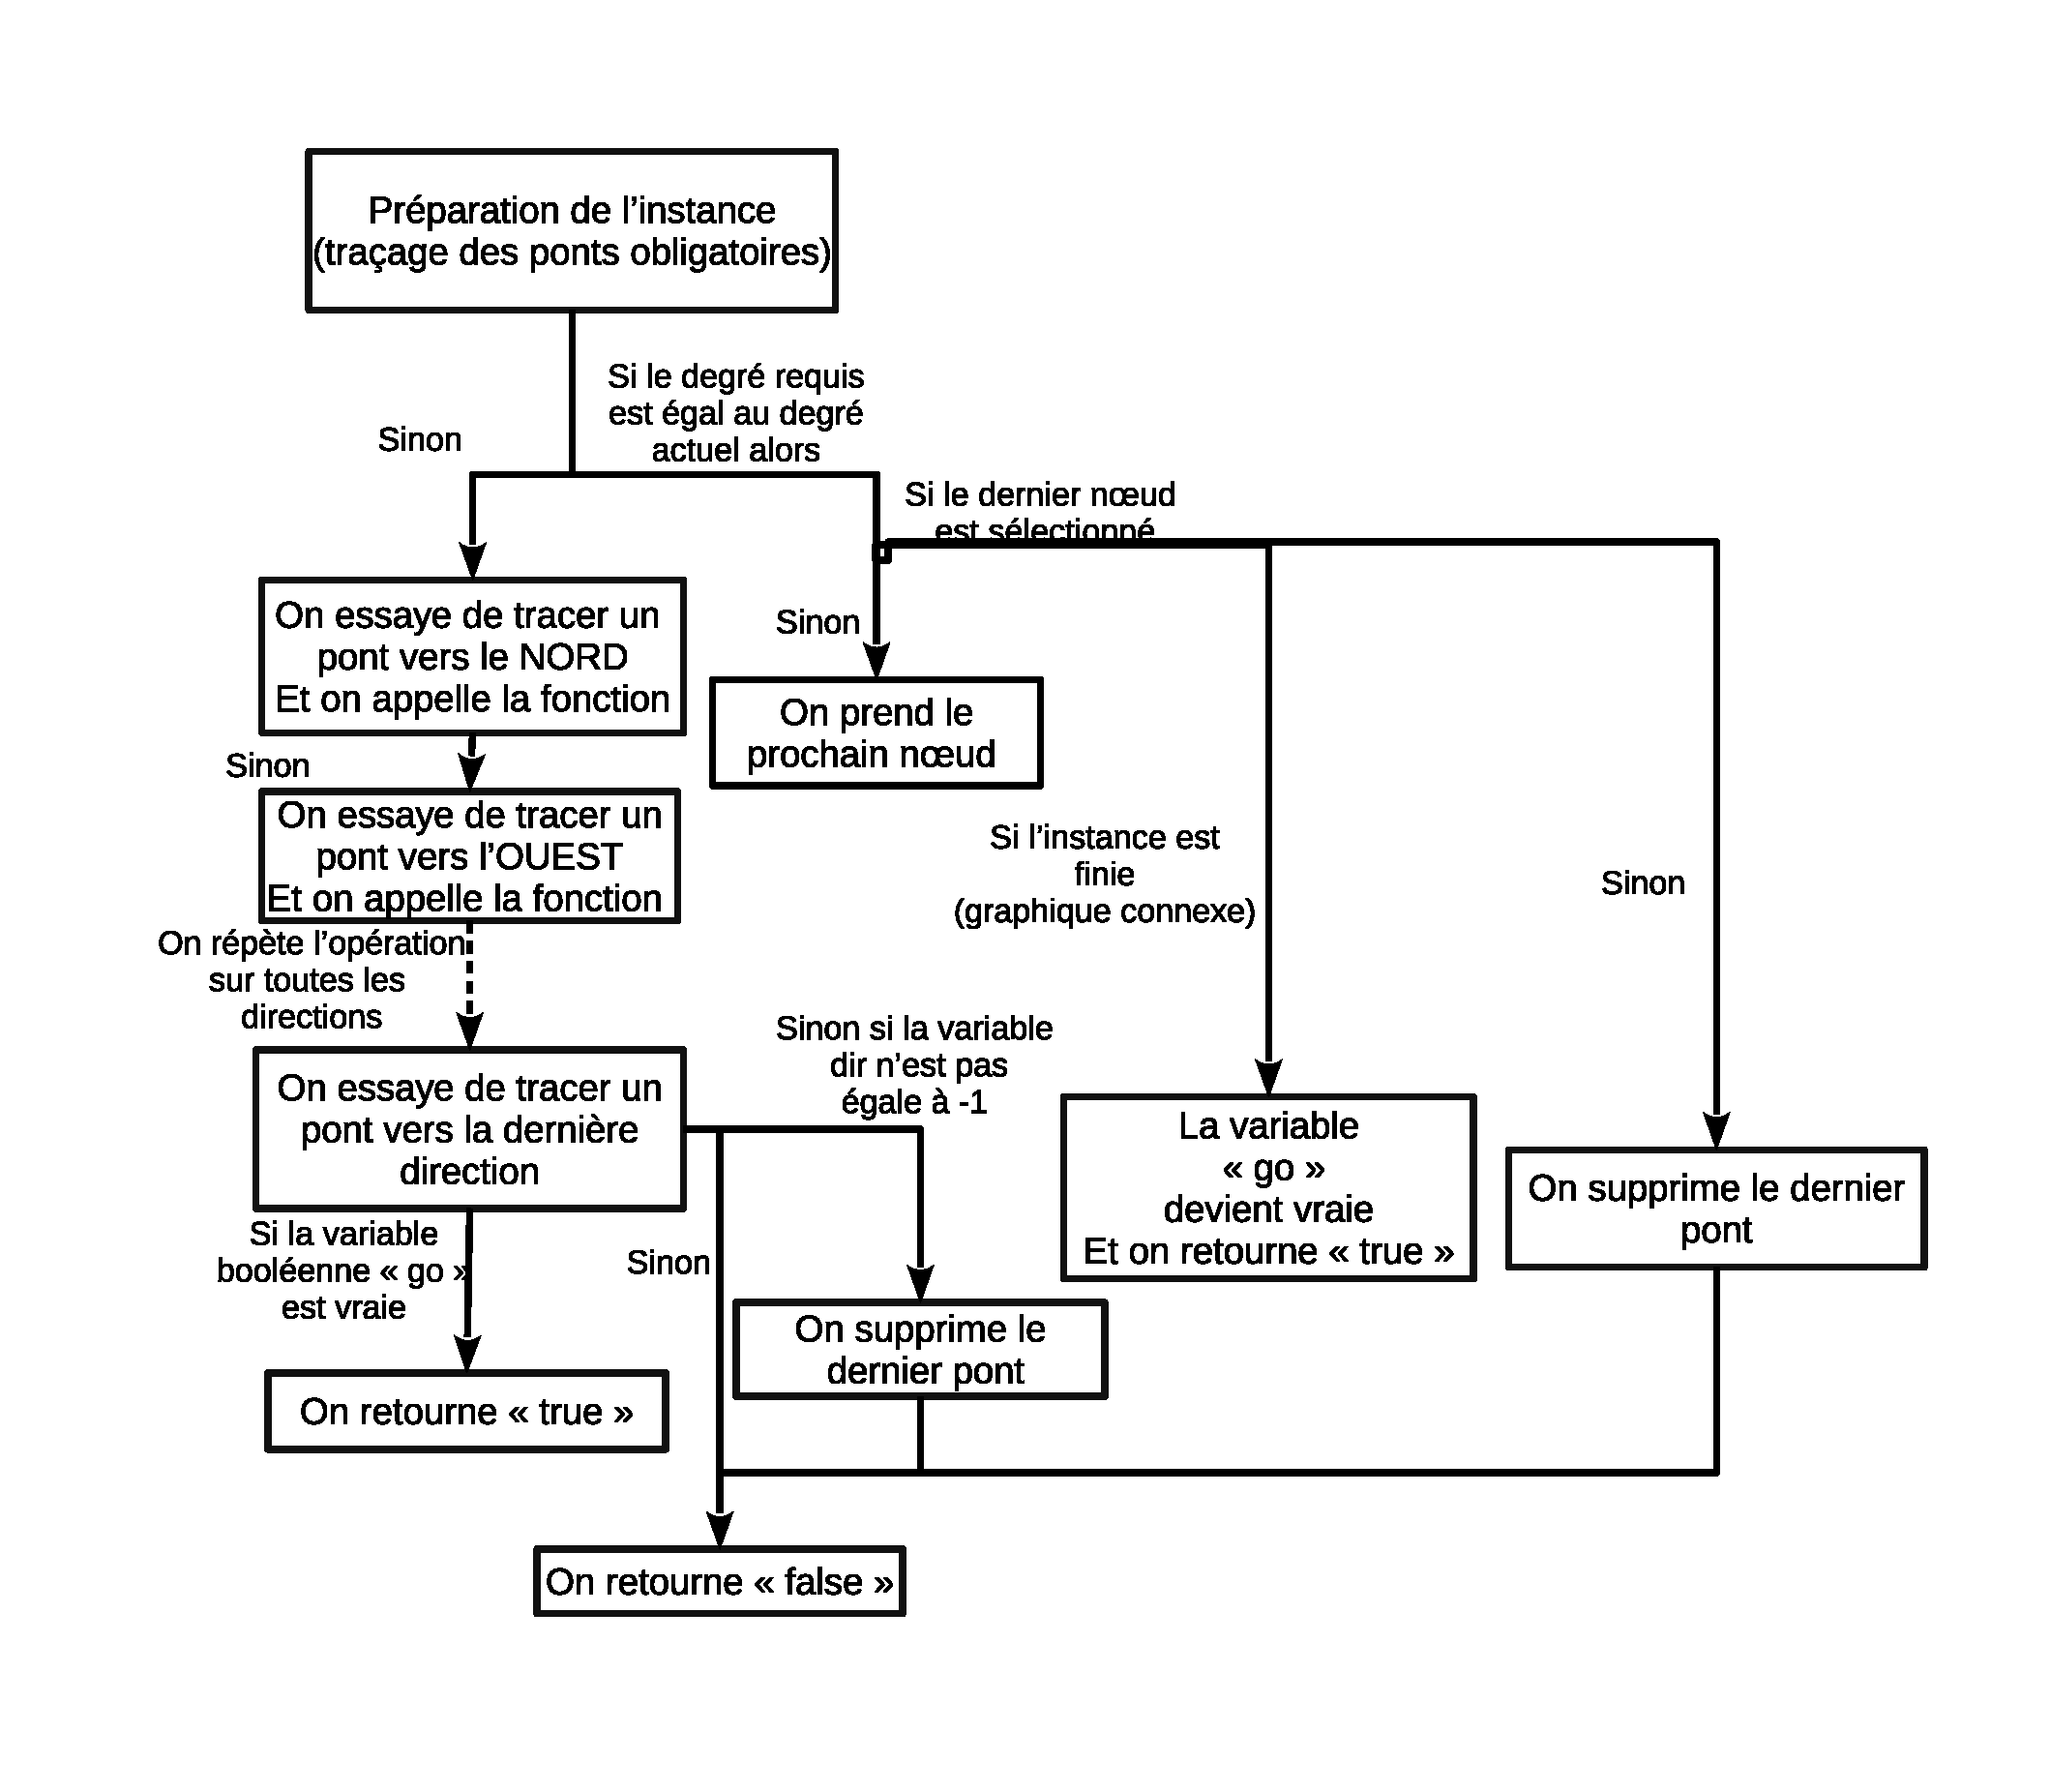
\includegraphics[width = 1.00\textwidth]{explication_solveur.eps}
\paragraph{Explication du graphique:\newline}
La préparation de l'instance consiste à tracer les ``ponts obligatoires'',cela concerne les îles qui n'ont qu'une possibilité de liens,
on a déterminé plusieurs cas:\newline
-Deux îles ne peuvent pas se completer totalement mutuellement, celà formerait un bloc connexe.\newline
-Si une île a un nombre de ponts possible maximum (en fonction des voisins possiblement atteignable) égale à son degré requis on doit tracer tout ses ponts.\newline

Les arguments de la fonction sont:\newline
-l'instance de jeu (g)\newline
-le numéro de l'île où nous allons appliquer nos opérations (node\_num)\newline
-la direction du dernier pont posé utile quand on dépile pour retirer le dernier pont (dir)\newline
-une variable indiquant si la solution a été trouvée (go)\newline

\paragraph{Possibilité d'amélioration:\newline}
Pour améliorer ce solveur on pourrait refaire le processus de ``ponts obligatoire'' à chaque fois que l'on fait une action mais celà implique d'avoir une sauvegarde de l'état du jeu pour que lorsque l'on dépile on puisse retirer les ponts posés par ce processus. On pourrait aussi améliorer 

\newpage
\section{Interface graphique}
\newpage
\section{Bonus: Portabilité sur Android}
\newpage

\end{document}
